\documentclass[journal,twoside,web]{ieeecolor}
\usepackage{generic}
% \usepackage{cite}
\usepackage{amsmath,amssymb,amsfonts}
\usepackage{bbm}
\usepackage{algorithmic}
\usepackage{graphicx}
\usepackage{textcomp}

\DeclareMathOperator*{\argmax}{argmax} % thin space, limits underneath in displays

% https://github.com/James-Yu/LaTeX-Workshop/wiki/FAQ#how-to-pass--shell-escape-to-latexmk
\usepackage{svg}

\usepackage{booktabs}
\usepackage{xcolor}
\usepackage{colortbl}
\usepackage{rotating}
\usepackage{multirow}

\usepackage{biblatex} %Imports biblatex package
\addbibresource{zotero.bib} %Import the bibliography file


% \def\BibTeX{{\rm B\kern-.05em{\sc i\kern-.025em b}\kern-.08em
%     T\kern-.1667em\lower.7ex\hbox{E}\kern-.125emX}}




\markboth{\journalname, VOL. XX, NO. XX, XXXX 2017}
{Author \MakeLowercase{\textit{et al.}}: Point-process based representation learning for Electronic Health Records}
\begin{document}
\title{Point-process based representation learning for Electronic Health Records}
\author{Hojjat Karami, \IEEEmembership{Fellow, IEEE}, Anisoara Ionescu, and David Atienza, \IEEEmembership{Member, IEEE}
\thanks{This paragraph of the first footnote will contain the date on 
which you submitted your paper for review. It will also contain support 
information, including sponsor and financial support acknowledgment. For 
example, ``This work was supported by DigiPredict Grant BS123456.'' }
\thanks{H. Karami is with the EPFL, Lausanne, Switzerland (e-mail: hojjat.karami@epfl.ch). }
\thanks{S. B. Author, Jr., was with Rice University, Houston, TX 77005 USA. He is 
now with the Department of Physics, Colorado State University, Fort Collins, 
CO 80523 USA (e-mail: author@lamar.colostate.edu).}
\thanks{T. C. Author is with 
the Electrical Engineering Department, University of Colorado, Boulder, CO 
80309 USA, on leave from the National Research Institute for Metals, 
Tsukuba, Japan (e-mail: author@nrim.go.jp).}}

\maketitle


\begin{abstract}

    Irregular sampling of time series in electronic health records (EHRs) presents a challenge for model development. In addition, the pattern of missingness for certain clinical variables is not random, but rather determined by clinicians' decisions and the patient's state. 
Point process is a mathematical framework for handling event sequence data that is consistent with irregular sampling. 
We propose \emph{NPP4EHR}, a deep neural network that can learn patient representations from irregularly sampled time series using the neural point process framework. We conducted various experiments to demonstrate the effectiveness of event and state encoding for characterizing conditional intensity functions, as well as for downstream prediction tasks, using two healthcare databases. 
Our proposed transformer event encoder outperforms state-of-the-art models in commonly used event sequence databases, as evidenced by its superior performance in negative log-likelihood and next-event prediction. Furthermore, we demonstrated the usefulness of state encoding for improved conditional intensity function characterization, as well as event encoding for better representation learning in downstream tasks, using two real-world healthcare datasets.
We propose that our model could be leveraged for better representation learning in EHRs.

\end{abstract}

\begin{IEEEkeywords}
    electronic health records (EHRs), Point Process, irregular sampling, informative missingness,
\end{IEEEkeywords}


\section{Introduction}
\label{sec:intro}

[ML in healthcare] Machine learning has the potential to revolutionize healthcare by leveraging vast amounts of data available in electronic health records (EHRs) to develop more accurate clinical decision support systems. EHRs store patient health information, such as medical history, medications, lab results, and diagnostic images, which can be used as input for machine learning algorithms to identify patterns and associations that could inform more precise diagnoses, better treatment plans, and earlier interventions. Clinical decision support systems that use machine learning can provide real-time, evidence-based recommendations to healthcare providers, reducing errors and improving patient outcomes.

[irregular sampling challenge] One of the data challenges for machine learning (ML) when using electronic health records (EHRs) is irregular sampling. EHR data is often collected at different times and frequencies, depending on a patient's healthcare needs and visit schedules, which can result in uneven and irregularly sampled time series data. Asynchronous and incomplete observation of certain clinical variables can also be regarded as missingness in the data.

missingness in tabular and time series.

[sources of missingness] The sources of missing data in EHRs must be carefully understood. For instance, lab measurements are usually ordered as part of a diagnostic work-up, and the presence or absence of a data point conveys information about the patient's state \cite*{ghassemiReviewChallengesOpportunities2020}.

[imputation methods] Imputation techniques are widely used in electronic health records (EHRs) to handle missing data. Imputation refers to the process of filling in the missing data with plausible values based on the available information. There are several imputation techniques available, each with its strengths and weaknesses. For example, mean imputation replaces missing values with the mean of the available values in the same column, while regression imputation uses a regression model to estimate the missing values based on the relationship between the variables. Other popular imputation methods include multiple imputations, hot deck imputation, and k-nearest neighbors imputation. The choice of imputation technique depends on the type and amount of missing data, as well as the goals of the analysis. Regardless of the technique used, it is important to carefully consider the impact of imputed values on the analysis and to report the imputation method used in the results.https://www.overleaf.com/project/63c00678bca7836b32514494

There exist several ML frameworks that are inherently compatible with the missing or irregularly-sampled data such as Gaussian process and recurrent neural networks.
Deep learning models that can handle irregularly sampled time series are crucial in many real-world applications, including stock market predictions, speech recognition, and medical diagnosis. These models must be able to process data that is not evenly spaced, which is common in time-sensitive applications. One popular deep learning architecture that can handle irregularly sampled time series is the Recurrent Neural Network (RNN). RNNs are well-suited for this task because they can process sequential data, taking into account not only the current input but also the previous inputs. 
Another architecture that can handle irregularly sampled time series is the Convolutional Neural Network (CNN), which can extract features from the data and then pass the processed data to an RNN for further analysis. Additionally, Attention Mechanisms can be integrated into RNNs and CNNs to help the model focus on important features in the data. These deep learning models offer a powerful toolset for handling irregularly sampled time series and providing useful insights into this type of data.
However, it is important to note that these models do not explicitly account for the fact that the absence of some data points can convey unique information, and it is important to carefully consider the sources of missingness in the data.

% Deep learning models that are compatible with irregularly sampled time series are important in many real-world applications, such as stock market predictions, speech recognition, and medical diagnosis. These models need to be able to handle data that is not evenly spaced, as is often the case in time-sensitive applications. One popular deep learning architecture that can handle irregularly sampled time series is the Recurrent Neural Network (RNN). RNNs are well-suited for this task because they can process sequential data, taking into account not only the current input but also the previous inputs. Another architecture that can handle irregularly sampled time series is the Convolutional Neural Network (CNN), which can be used to extract features from the data and then pass the processed data to an RNN for further analysis. Additionally, Attention Mechanisms can be integrated into RNNs and CNNs to help the model focus on important features in the data. Overall, these deep learning models offer a powerful toolset for handling irregularly sampled time series and provide useful insights into this type of data. However, these models do not explicitly take into account the fact wether the absence of some datapoints could convey some unique information.




Point process is the mathematical framework for describing the distribution of events in time or space. These events can be occurrences of earthquakes, nerve impulses, customer purchases, or anything else that can be counted or measured.
In healthcare, lab measurements can be regarded as sequence of events that are ordered by clinicians. At the core of point process is the defintion of conditional intensity functions and the corresponding log-likelihood which simultanously models the occurence of events using the history of past events.

Point process is a mathematical framework for describing the distribution of events in time or space. These events can be occurrences of earthquakes, nerve impulses, customer purchases, or anything else that can be counted or measured. In healthcare, lab measurements can be regarded as a sequence of events that are ordered by clinicians.
At the core of the point process is the definition of conditional intensity functions and the corresponding log-likelihood, which simultaneously models the occurrence of events using the history of past events. The conditional intensity function represents the instantaneous rate of event occurrence, given the history of past events. This function can be used to predict the probability of future events, which is particularly useful in healthcare applications such as predicting disease onset or detecting adverse events.

% More recently, neural Point Processes (NPP) have been developed for better characteriztion of CIFs by leveraing the power of deep neural networks. These models can be used for tasks such as predicting future events, estimating the rate of event occurrence, or identifying correlations between events. They offer a flexible and powerful way to analyze point process data, as they can handle complex dependencies between events and incorporate prior knowledge about the process. Traditioaly, a point process encodes timestamp and type of events, however, it is common in healtcare to have additional sources of information that could be useful for CIF characterization. For example the absolute value of patients vital signs might be predictive for next event prediction.

More recently, Neural Point Processes (NPP) have been developed to better characterize Conditional Intensity Functions (CIFs) by leveraging the power of deep neural networks. These models can be used for tasks such as predicting future events, estimating the rate of event occurrence, or identifying correlations between events. They offer a flexible and powerful way to analyze point process data, as they can handle complex dependencies between events and incorporate prior knowledge about the process.
Traditionally, a point process encodes the timestamp and type of events. However, in healthcare, additional sources of information can be available that could be useful for CIF characterization. For example, the absolute value of a patient's vital signs might be predictive for next-event prediction. NPP models can incorporate such information by using event and state encoders that can learn to extract relevant features from the input data.

Our proposed model, NPP4EHR, is a deep learning model for electronic health records (EHRs) that is based on point process theory. It consists of two modules: a transformer event encoder, which is designed to handle the missingness patterns of certain laboratory values, and a deep attention module for encoding all other available data. Both modules can be jointly learned by using appropriate loss functions for conditional intensity function (CIF) characterization and any downstream task.

We have conducted extensive experiments on existing event sequence data to demonstrate the effectiveness of our improved transformer event encoder in comparison to existing methods. Furthermore, we have shown that encoding states can reduce the negative log-likelihood (NLL) in two EHR datasets and, in some cases, lead to better performance for next event prediction. Overall, our proposed model offers a powerful tool for handling the irregularly sampled time series data present in EHRs and has the potential to improve representation learning in this domain.
The contributions of this paper are:
\begin{itemize}
    \item An improved transformer event encoder that can effectively handle missingness patterns in certain laboratory values and has been validated in baseline datasets.
    \item A deep attention module for encoding all available patient data, which has been shown to improve CIF characterization for laboratory values.
    \item Leveraging transformer event encoder in downstream tasks for better representation learning of patient's EHR
\end{itemize}



\section{Background}
\label{sec:Background}










\subsection{Temporal point process}


A temporal point process is a stochastic process that models a sequence of events in a continuous time domain. Consider event sequence data  $\mathcal{D}=\{\mathcal{S}_{i}\}_{i=1}^N$ where $N$ is the total number of samples and each sample $\mathcal{S}_{i}$ is represented as a sequence of events $\mathcal{S}_{i}=\{(t_i,e_i)\}_{j=1}^L$, where $L$ is the total number of occurred events, $t_j$ is the event's timestamp, and $e_j \in \mathbb{R}^M $ is the binary representation of event marks (multi-class or multi-label). Furthermore, the history of events at time $t$ is denoted as $\mathcal{H}_t=\{(t_j,e_j):t_j<t \}$.


The core idea of the point process framework is the definition of conditional intensity functions (CIFs) which is the probability of the occurrence of an event of type $m$ in an infinitesimal time window $[t,t+dt)$:

\begin{equation} \label{eq:lambda_def}
   \lambda_m^{*}(t)=\lim \frac{P(  \text{event of type m in } [t,t+\Delta t) |   \mathcal{H}_t  )}{\Delta t} 
\end{equation} 

Here, $*$ denotes conditioning on the history of events$\mathcal{H}_t$. The Multivariate Hawkes process is the traditional approach to characterize CIFs by assuming a fixed form of intensity to account for the additive influence of an event in the past:

\begin{equation} 
    \lambda_m^{*}(t)= \mu_m + \sum_{(t^{\prime},e^{\prime})\in \mathcal{H}_t} \phi(t-t^{\prime})
 \end{equation} 

 where $\mu \ge 0 $, aka base intensity, is an exogenous component that is independent of history, while $\phi(t)>0$, excitation function, is an endogenous component depending on the history that shows the mutual influences. The excitation function can be characterized using exponentials, or linear combination of $M$ basis functions \cite*{xuLearningGrangerCausality2016}.



 \subsection{Parameter Estimation}

 Based on the conditional intensity function \ref*{eq:lambda_def}, it is straightforward to derive conditional probability density function $p^{*}_{m}(t)$ in the interval $(t_j, t_{j+1}]$:
 
 \begin{equation} 
     p_m^{*}(t)=\lambda_m^{*}(t) \exp \left[-\sum_{m=1}^{M} \int_{t_j}^{t_{j+1}}\lambda_m^{*}(s)ds\right]
  \end{equation}
  
 
  The parameters of the point process can be learned by Maximum Likelihood Estimation (MLE) framework. However, more advanced methods such as adversarial learning, and reinforcement learning have also been proposed.
 
 In the multi-class setting, the log-likelihood (LL) of a point process for a single event sequence $\mathcal{S}_{i}$ is defined as:
 
 \begin{multline} \label{eq:CIF-mc}
     \log p_{mc}(\mathcal{S}_{i})  =  \sum_{j = 1}^{L}\sum_{m = 1}^{M} \mathbbm{1}(e_j=m)   \log p_m^{*}(t_j) \\   
     = \sum_{j = 1}^{L}\sum_{m = 1}^{M} \mathbbm{1}(e_j=m)   \log \lambda_m^{*}(t_j)\\
     -\sum_{m = 1}^{M} \left(   \int_{t_1}^{t_L}  \lambda_m^{*}(s) \,ds  \right)
 \end{multline} 
 
 Here, $\mathbbm{1}$ is the indicator function. The log-likelihood can be understood using the following two facts. First, the quantity $\lambda_k^{*}(t)dt$ corresponds to the probability of observing an event of type $k$ in the infinitesimal interval $[t_j,t_j+dt]$ conditioned on the past events $\mathbb{H}_{t_j}$. Second, we can compute the probability of not observing any events of type $k$ in the rest of the interval $[t_1,t_L]$ as $\exp \left(-\int_{t_1}^{t_L}  \lambda_m^{*}(s) ds\right)$.
 
 However, in many cases, such as in EHRs, it is common to have co-occurring events. To handle this issue, \cite*{enguehardNeuralTemporalPoint2020} proposed using a binary cross-entropy function:
 
 
 \begin{multline} \label{eq:CIF-ml}
     \log p_{ml}(\mathcal{S}_{i}) = \log p_{mc}(\mathcal{S}_{i}) \\
     + \sum_{m = 1}^{M} (1-\mathbbm{1}(e_j=m)) \log \left(1-p_m^{*}(t_j)  \right)
 \end{multline} 
 
 
 % \begin{multline} 
 %     -\log p(\mathcal{S}_{i})  =  - \sum_{j = 1}^{L}\sum_{m = 1}^{M} 1(e_j=m)   \log \lambda_m^{*}(t_j) \\   
 %     + \sum_{m = 1}^{M} \left(   \int_{0}^{T}  \lambda_m^{*}(s) \,ds  \right)\\
 %     - \sum_{j = 1}^{L}\sum_{m = 1}^{M} (1-1(e_j=m)) \log \left(1-\lambda_m^{*}(t_j) \exp \left( - \int_{0}^{T}  \lambda_m^{*}(s) \,ds  \right) \right)
 % \end{multline} 
 
%  It should be noted that the real advantage of point process is modeling non-event likelihoods in the form of integrals. If we neglect the integrals, we would achieve the cross-entropy and binary cross entropy loss in the multi-class and multi-label settings respectively for the prediction of next mark given history of events.


 It is important to note that the main advantage of point processes lies in their ability to model non-event likelihoods in the form of integrals. If we neglect the integrals, we would end up with the cross-entropy and binary cross-entropy loss in the multi-class and multi-label settings, respectively, for predicting the next mark given the history of events.
 
 Another approach is the marked case, which assumes that the marks and timestamps are conditionally independent given $\mathcal{H}_t$:
 
 \begin{multline} \label{eq:CIF-marked}
     \log p_{marked}(\mathcal{S}_{i}) =    
     \sum_{j = 1}^{L}\sum_{m = 1}^{M} \mathbbm{1}(e_j=m)   \log p^{*}(e_j=m) \\
     +\sum_{j = 1}^{L}\lambda^{*}(t_j) - \int_{t_1}^{t_{L}}\lambda^{*}(t^{\prime})dt^{\prime}  
 \end{multline} 
 
 This marked case is basically an autoencoder for next mark prediction with a single dimension point process for timestamps only.
 
 

\subsection{Neural temporal point process}

Encoder-decoder architectures have proven to be effective in many applications. The main idea of a neural temporal point process (NTPP) is to first encode the history of events until $t_j$ using a neural network architecture $h_j=Enc(\mathcal{H}_{j+1};\theta)$. Then it tries to estimate $m$ CIF using a different decoder architecture $\lambda^*_m(t)=Dec(h_j;\phi)$ for $ t \in (t_j,t_{j+1}]$.

% Initial works have used recurrent encoders such as RNN, GRU or LSTM [refs] in which the hidden state gets updated after the arrival of a new event as $h_{j+1}=Update(h_j,(t_j,e_j))$. The main advantage is that they allow us to compute history embeddings in $O(L)$ time, however, they are prone to neglect long-term inter-event influences. On the other hand, set aggregation encoders directly encode all past events into a history embedding. Adopting an attention mechanism is one such way that can capture long-term influences and can be trained in parallel as well which makes it more computationally efficient. For example, \cite*{zuoTransformerHawkesProcess2020a} proposed Transformer Hawkes Process (THP) that adopts a transformer architecture for event encoding.

Initial works have utilized recurrent encoders such as RNN, GRU, or LSTM, where the hidden state is updated after the arrival of a new event as $h_{j+1}=Update(h_j,(t_j,e_j))$. The main advantage of these models is their ability to compute history embeddings in $O(L)$ time. However, they are susceptible to ignoring long-term inter-event dependencies.
In contrast, set aggregation encoders encode all past events directly into a history embedding. One approach to capture long-term dependencies is to use an attention mechanism, which can be trained in parallel and is more computationally efficient. For instance,\cite{zuoTransformerHawkesProcess2020a} proposed Transformer Hawkes Process (THP), which adopts a transformer architecture for event encoding.

The learned event embeddings can be later used for estimating conditional intensity functions, cumulative conditional intensity functions or probability density functions.


\subsection{Deep learning for irregularly sampled data}
An irregularly sampled data can be denoted as $\mathcal{D}=\{\mathcal{U}_i\}_{i=1}^{N}$ where $N$ is number of samples and each sample is represented as sequence of tuples $\mathcal{U}_i=\{(t_p,k_p,v_p)\}_{p=1}^{P}$ where $P$ is the total number of observations and $t_p, k_p, v_p$ represents the time, modality and value of $p$-th observation respectively.

Recurrent neural networks can naturally deal with sequential data. These models can be made compatible with irregularly sampled data by adding a strategy to consider time.

\section{Related Works}
\label{sec:Related Works}

We focus on Neural point process models based on attention mechanisms that can potentially address the problems of slow serial computing and loss of long-term information. In addition, attention weights bring interpretability and can show peer influences between events. Self-attentive Hawkes Process (SAHP) \cite*{zhangSelfAttentiveHawkesProcess2020} proposes a multi-head attention network as the history encoder. In addition, they use a sofplus function that can capture both excitation and inhibition effects. Similarly, Transformer Hawkes Process (THP) \cite*{zuoTransformerHawkesProcess2020a} adopts the transformer architecture \cite*{vaswaniAttentionAllYou2017} with time encodings for event embeddings. They have introduced softplus function that can only capture mutual excitations between events. In an interesting study \cite*{enguehardNeuralTemporalPoint2020}, researchers studied different combinations of encoders (self-attention and GRU) and decoders and simulated on various datasets for comparison. They demonstrated that attention-based TPPs appear to transmit pertinent EHR information and perform favorably compared to existing models. One gap in the current literature is that they don't have any means for encoding additional information that can be useful for the characterization of CIFs. For example, in EHRs there are many information in addition to clinical events that could be useful

Recurrent neural networks have been modified to consider irregularly sampled time series. For example, GRU-D \cite*{cheRecurrentNeuralNetworks2018} adapts GRU to consider missingness patterns in the form of feature masks and time intervals to achieve better prediction results. RETAIN \cite*{choiRETAINInterpretablePredictive2017} is based on a two-level neural attention model that is specifically designed for EHRs data. SeFT \cite*{hornSetFunctionsTime2020} is based on recent advancements in differentiable set function learning, extremely parallelizable with a beneficial memory footprint, thus scaling well to large datasets of long time series and online monitoring scenarios. Their use of aggregation function is similar to transformers that compute the embeddings of set elements independently, leading to lower runtime and memory complexity of $O(n)$. Although these models are nearly end-to-end that eliminate the need for an imputation pipeline, it is still unclear how much they are affected by the missingness pattern in EHRs. In addition, they do not explicitly model the missingness pattern in the data.



\section{Proposed Model}
\label{sec:Proposed Model}


\begin{figure*}[!t]
\centerline{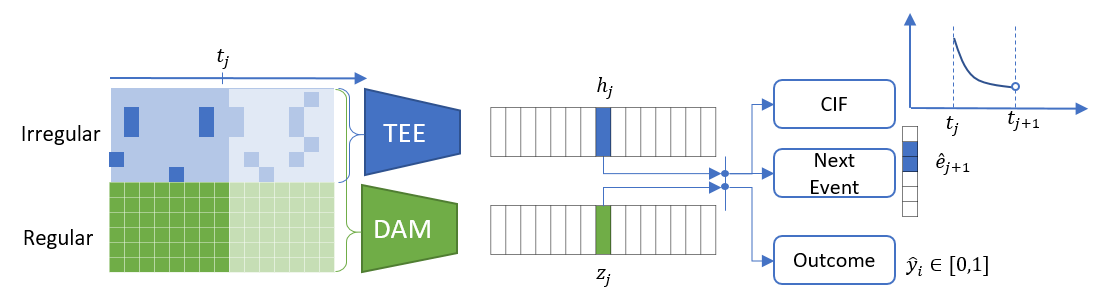
\includegraphics{images/model_arch.png}}
\caption{Magnetization as a function of applied field.
It is good practice to explain the significance of the figure in the caption.}
\label{fig1}
\end{figure*}

The proposed model, NPP4EHR, consists of two modules for encoding a dataset with both event sequence data and irregularly sampled time series. The schematic of the model is depicted in \ref*{fig1}.

 The key advantage of our proposed model is to combine a transformer-based event encoder (TEE) with a deep attention module (DAM) that can handle an irregularly sampled time series for any downstream prediction task. The data is represented as $\mathcal{D}=\{(\mathcal{S}_i,\mathcal{U}_i)\}_{i=1}^{N}$, where $\mathcal{S}_i$ and $\mathcal{U}_i$ are event sequence data and irregular time series for the $i$-th sample as described in previous section.

\subsection{Event Encoder}
We use a transformer event encoder similar to THP \cite*{zuoTransformerHawkesProcess2020a} with minor modifications for time encoding.
In the first step, we embed all event marks as $E_{emb}=E \times W_{emb}$, where $E_i \in \mathbb{R}^{L \times M}$ is the binary encoding matrix of all event marks (multi-label or multi-class), and  $ W_{emb} \in  \mathbb{R}^{M \times d_{emb} }  $ is the trainable embedding matrix. In addition, we encode vector of timestamps $t=[t_1,t_2,...,t_L] $ to $Z=[z(t_1),z(t_2),...,z(t_L)]\in \mathbb{R}^{L \times d_{time}}$ using following transformation formula:

\begin{equation}\label{eq:time-encoding}
    [z(t_j)]_{k} = 
     \begin{cases} 
        \cos\left(  \frac{t_j}{\mathcal{T}^{(k-1)/d_t} }  \right) & \text{if } k \text{ is odd}\\
        \sin\left(  \frac{t_j}{\mathcal{T}^{k/d_t} }  \right) & \text{if } k \text{ is even}

        \end{cases} 
\end{equation} 
Here, $\mathcal{T}$ is representing the maximum time scale. This transformation is very similar to positional encodings in transformers \cite*{vaswaniAttentionAllYou2017}, where the index is substituted by the timestamp. Contrary to THP and original positional encoding that considers $d_{emb}=d_{time}$ and adds up time encoding to the event embedding, we propose to concatenate these two vectors:

\begin{equation}
    X_{ev}=[W_{emb}, Z] \in \mathbb{R}^{L \times (d_{emb}+t_{emb})}
\end{equation}



% In the second step, timestamps should be encoded and added to the event embedding, however, we propose to concatenate time encodings that can lead to better characterization of conditional intensity functions. Finally, the input of the transformer encoder will be $X_{emb}=[E_{emb}, T_{emb}] \in \mathbb{R}^{L \times (d_{emb}+t_{emb})}$.

Finally, we use the standard transformer architecture to encode embedded events $X_{ev}$ into the encoded matrix  $ H=(h_1, ..., h_j, ..., h_L) $. It is important to use an appropriate mask matrix to prevent information leakage from the future to the past. In this case, $h_j$ should contain all available information until the occurrence of $j$-th event.






\subsection{State Encoder}

We use a deep attention module \cite*{hornSetFunctionsTime2020} for encoding all additional information including irregularly sampled time series. Each observation is represented by $u_p=(z(t_p), v_p, m_p)$ where $z(t_p)$ is the same transformation for time encoding in equation \ref{eq:time-encoding}.% we define attention $a(\mathcal{U}_k,s_k )$

We define $\mathcal{U}_p$ to be the set of the first $p$ observations.
The goal is to calculate the attention weight $a(\mathcal{U}_p,u_k ), k \leq p$ that is the relevance of $k$-th observation $u_k$ to the first $p$ observed values $\mathcal{U}_p$.
This is achieved by computing an embedding of the set elements using a smaller set functions $f^{\prime}$, and projecting the concatenation of the set representation and the individual set element into d-dimensional space:



\begin{equation}\label{eq:fprime}
   f^{\prime}(\mathcal{U}_p) = g^{\prime} \left(  \frac{1}{|p|} \sum_{u_k \in \mathcal{U}_p}  h^{\prime}(u_k;\theta^{\prime}) ;\rho^{\prime}\right) 
\end{equation}

Here, we compute the mean of the first $p$ observations after passing the first $p$ observations through a multilayer perceptron (MLP) neural network ($h^{\prime}(u_k;\theta^{\prime})$). Finally, a second transformation using $g^{\prime}$ is performed to obtain embeddings $f^{\prime}(\mathcal{U}_p) \in \mathbb{R}^{d_{g^{\prime}}}$.


Then we can compute key values ($ K_p$) using key matrix $W^k \in \mathbb{R}^{(d_{g^{\prime}}+d_s) \times d_{prod}}$:


\begin{equation}
    K_p=[f^{\prime}(\mathcal{U}_p), u_p]^T W^K   
\end{equation}

Then using a query vector $w^q \in \mathbb{R}^{d_{prod}}$, we compute the desired attnetion weight in this way:

\begin{equation}
    a(\mathcal{U}_p,u_k)=  softmax(\frac{K_p.w^q}{\sqrt{d}  })
\end{equation}


Finally, we compute a weighted aggregation of set elements using attention weights similar to equation \ref*{eq:fprime}:

\begin{equation*}
    y_p=f(\mathcal{U}_p) =     
    g\left(
    \sum_{u_k \in \mathcal{U}_p}  a(\mathcal{U}_p,u_k)h(u_k;\theta);\rho 
    \right) 
\end{equation*}

We regard $y_p \in \mathbb{R}^{d_g}$ as the representation of first $p$ observations.

The matrix $Y=[y_1,y_2,...,y_P] \in \mathbb{R}^{P \times d_g}$ keeps the entire representions of the data. To use state information for CIFs characterization, we down-sample $Y$ to $Y^{\prime}=[y^{\prime}_1,y^{\prime}_2,...,y^{\prime}_L]  \in \mathbb{R}^{L \times d_g}$ where $ y^{\prime}_j=y_p \text{ where } p=\argmax_{t_p \leq t_j} p$.

Without loss of generality, we can consider multiple heads by adding an additional dimension to keys and queries.

% We need to combine event embeddings $ H_{L \times d_e}$ and state embeddings $Y_{P \times d_g}$, however, the length of each matrices does not match. As a result, we consider the reduced version of state matrix as below:

% \begin{equation*}
%     y^{\prime}_j=y_p \text{ where } p=\argmax_{t_p \leq t_j} p
% \end{equation*}








% \subsection{All formulas}

% \begin{equation*}
%     \begin{cases} 


% f^{\prime}(\mathcal{S}_p) = g^{\prime} \left(   
%  \frac{1}{p} \sum_{s_k \in \mathcal{S}_p}  h^{\prime}_{\theta}(s_k) 
% \right) \\


% K_p=[f^{\prime}(\mathcal{S}_p), s_p]^T W^K \\
% e_p=\frac{K_p.w^q}{\sqrt{d}  }\\


% a(\mathcal{S}_p,s_k)=\frac{\exp (e_p)}{\sum_{k\leq p} \exp (e_k)  } \\


% f(\mathcal{S}_p) = \sum_{s_k \in \mathcal{S}_p}  a(\mathcal{S}_p,s_k)h_{\theta}(s_k) \\


% z_p=g_{\psi}\left(         f(\mathcal{S}_p)         \right) \\



% \end{cases} 
% \end{equation*}


% \begin{equation}
%     \lambda_k(t|\mathcal{H}_t ) = f_k\left(\alpha_k \frac{t-t_j}{t_j}+\mathbf{w}_k^T \mathbf{x}_{enc}(t_j)+\mathbf{y}_k^T \mathbf{s}_{enc}(t_j) +b_k   \right)
% \end{equation}

% \begin{equation}
%     \lambda_k(t|\mathcal{H}_t ) = f_k\left(\alpha_k \frac{t-t_j}{t_j}+\mathbf{w}_k^T \mathbf{x}_{enc}(t_j)+b_k   \right)
% \end{equation}

\subsection{Event Decoder}
Once we obtain a representation of a patient using embedded events and states, we can try to parameterize conditional intensity functions (CIFs) of the events.

In neural point process literature, many approaches have been propose to decode either conditional or cumulative intensity function. We will use a decoder similar to \cite*{zhangSelfAttentiveHawkesProcess2020} as it can model both exciting and inhibiting effects for modeling CIFs.

% \begin{gather*} 
%    \mu_{m,i+1}=gelu(h_{i+1}W_{m,\mu}), 
% \end{gather*}

\begin{gather} 
    \mu_{m,j}=gelu(h_{j}W_{m,\mu}  +  y^{\prime}_{j}W_{m,\mu}), \\ 
    \eta_{m,j}=gelu(h_{j}W_{m,\eta}  +  y^{\prime}_{j}W_{m,\eta}), \\
    \gamma_{m,j}=gelu(h_{j}W_{m,\gamma}  +  y^{\prime}_{j}W_{m,\gamma}),
    \end{gather}

Finally, we can express the intensity function as follows:

\begin{multline}
    \lambda_m(t)=\text{softplus}(\mu_{m,j}+\\
    (\eta_{m,j}- \mu_{m,j}) \exp(-\gamma_{m,j}(t-t_j))    ),
\end{multline}

for $t \in (t_j, t_{j+1}]$,where the $softplus$ is used to constrain the intensity function to be positive.


\subsection{Loss Function}

We define a multi-objective loss function as $ \mathcal{L}   =   \mathcal{L}_{CIF}   +   \beta \mathcal{L}_{state}$., where $\mathcal{L}_{CIF}$ could be one of equations \ref*{eq:CIF-mc},\ref*{eq:CIF-ml} or \ref*{eq:CIF-marked}, and $\mathcal{L}_{state}$ could be any desired loss function such as mean square error or cross-entropy depending on the task. $\beta$ is a coefficient that can be optimized during hyperparameter tuning.





\section{Experiments}
\label{sec:Experiments}

We perform various experiments to show the effectiveness of each component in our model.
\subsection*{Datasets}

% Table generated by Excel2LaTeX from sheet 'datasets'
\begin{table}[htbp]
    \centering
    \caption{Add caption}
      \begin{tabular}{ccccc}
      \toprule
      \toprule
      Dataset & Task  & \# classes & \# samples & Avg. length \\
      \midrule
      Stack Overflow & Multi-class & 22    & 6633  & 72 \\
      ReTweets & Multi-class & 3     & 24000 & 109 \\
      ReTweets & Multi-label & 3     & 20000 & 104 \\
      Synthea & Multi-label & 357   & 12000 & 43 \\
      Physionet 2012 & Multi-label & 25    & 12000 & 21 \\
      Physionet 2019 & Multi-label & 25    & 12000 & 21 \\
      \bottomrule
      \bottomrule
      \end{tabular}%
    \label{tab:data}%

  \end{table}%
  
  
  
  

\textbf{Synthea(\emph{SYN})}.
We used the Synthea simulator \cite*{walonoskiSyntheaApproachMethod2018} which generates patient-level EHRs using human expert-curated Markov processes. Here, we reused the already processed version of this data by \cite*{enguehardNeuralTemporalPoint2020}.

\textbf{ReTweets (\emph{RT})}.
The Retweets dataset contains sequences of tweets, where each sequence contains an origin tweet (i.e., some user initiates a tweet), and some follow-up tweets. We record the time and the user tag of each tweet. Further, users are grouped into three categories based on the number of their followers: “small”, “medium”, and “large”. We use two versions of this dataset for multi-class \cite*{zhangSelfAttentiveHawkesProcess2020} and multi-label \cite*{enguehardNeuralTemporalPoint2020} scenario.

\textbf{Stackoverflow (\emph{SO})} is a question-answering website. The website rewards users with badges to promote engagement in the community, and the same badge can be rewarded multiple times to the same user. We collect data in a two-year period, and we treat each user’s reward history as a sequence. Each event in the sequence signifies receipt of a particular medal. We used the same processed dataset in the literature \cite*{zuoTransformerHawkesProcess2020a}.

Furthermore, we consider two EHRs provided by physionet:

\textbf{Physionet 2012 Mortality Prediction Challenge (\emph{P12})}.
The 2012 Physionet challenge dataset \cite*{silvaPredictingInHospitalMortality},contains 12, 000 ICU stays each of which lasts at least 48 hours. For each stay, a set of general descriptors (such as gender or age) are collected at admission time. Depending on the course of the stay and patient status, up to 37 time series variables were measured (e.g. blood pressure, lactate, and respiration rate). While some modalities might be measured in regular time intervals (e.g. hourly or daily), some are only collected when required; moreover, not all variables are available for each stay.

\textbf{Physionet 2019 Sepsis Early Prediction Challenge (\emph{P19})}.
This dataset contains clinical data of about 40,000 patients in ICU \cite*{reynaEarlyPredictionSepsis2020}. Clinical data consist of demographics, vital signs and laboratory values as well as sepsis label in a one-hour time grid.


\subsection*{Experimental Setup}

In the first series of experiments, we compare our proposed model for point process modeling in three scenarios:

\begin{itemize}
    \item \emph{AE(next mark)} is a simple auto-encoder for predicting the next event from event embeddings without CIF characterization. The loss function is cross-entropy or binary cross-entropy for multi-class and multi-label datasets respectively. This scenario provides a baseline for other point process-based scenarios.
    \item \emph{PP(marked)} is a marked point process (\ref*{eq:CIF-marked}) where we assume marks and time stamps are independent.
    \item \emph{PP(multi-class or multi-label)} uses multi-class (\ref*{eq:CIF-mc}) or multi-label loss (\ref*{eq:CIF-ml}).
\end{itemize}

To show the utility of time concatenation, we also report the metrics for the summation case.

In the second series, we want to investigate the effectiveness of state encoding in addition to the events for real-world EHR datasets P12 and P19 in a multi-label setting. We regard the occurrence of certain laboratory variables as events that are based on clinicians' decisions (see Appendix). As a result, we consider two scenarios:

\begin{itemize}
    \item \emph{TEE}: Here, we only use the transformer event encoder (TEE) for CIFs characterization.
    \item \emph{TEE+DAM}: We further encode time stamps and values of all clinical variables through the deep attention module (DAM).
    \item \emph{TEE+noise}: To further investigate that the improved performance in the second scenario is not due to larger vector representation, we replace the DAM representations by a Gaussian noises vector ($\epsilon \sim \mathcal{N} (0,1)$).
\end{itemize}

In the last series of experiments, we investigate the utility of event encoding in a downstream supervised learning task. In particular, we try to predict mortality and sepsis shock as a binary outcome in P12 and P19 respectively. As a result, we compare (TEE+DAM) against the baseline (DAM) for outcome prediction.

We further split healthcare datasets (P12 and P19) into three settings to compare for generalizability across different centers:

\begin{itemize}
    \item single-center (sc): Training data is from the same center as the test data.  
    \item external evaluation (mc2): Training data is from all centers excluding the test data center:
    \item multi-center (mc1): Training data is from all available center
\end{itemize} 




\subsection*{Metrics}
We report log-likelihood normalized by the number of events (LL/\#events) as a goodness of fit for CIFs characterization \cite*{zhangSelfAttentiveHawkesProcess2020,zuoTransformerHawkesProcess2020a}. For the next event type prediction, we report the weighted measure of F1-score and area under the receiver operating characteristic curve (AUROC) in the multi-class and multi-label setting respectively. In the supervised learning task for binary prediction, we report F1-score and area under the precision-recall curve (AUPRC).

We use t-SNE (t-Distributed Stochastic Neighbor Embedding) for showing learned representations in the downstream tasks which is a machine learning algorithm used for visualizing high-dimensional data in a lower-dimensional space \cite*{maatenVisualizingDataUsing2008}.

To show the similarity of events in the learned representation, we first compute the measurement density of each laboratory variable during patient stay:

\begin{equation}
    d_{m}^{i}=  \frac{1}{t_L} \sum_{j=1}^{L} \mathbbm{1}(e_j=m),
\end{equation}

The mean of cosine similarities between the measurement density of a desired patient and its 10 nearest neighbors (in the embedding space) is computed (10-nnps).
\subsection*{Training Details}
To be completed.


\section{Results and Discussion}
\label{sec:Results and Discussion}


% In this section, we present our results regarding the advantage of state and event encoding.

\subsection{Preliminary comparison}




% Table generated by Excel2LaTeX from sheet 'time concat'
% Table generated by Excel2LaTeX from sheet 'time concat'
\begin{table*}[htbp]
    \centering
    \caption{Add caption}
      \begin{tabular}{ccccccccccccccc}
      \toprule
      \toprule
            &       & \multicolumn{8}{c}{TEEDAM}                                    &       &       &       &       &  \\
  \cmidrule{3-10}          &       & \multicolumn{2}{c}{AE (next-mark)} &       & \multicolumn{2}{c}{PP(single+mark)} &       & \multicolumn{2}{c}{PP (MC/ML)} &       & \multicolumn{4}{c}{Baselines} \\
  \cmidrule{3-4}\cmidrule{6-7}\cmidrule{9-10}\cmidrule{12-15}    Dataset & Metric & concat & sum   &       & concat & sum   &       & concat & sum   &       & Latent & SAHP  & THP   & GRU-CP \\
      \midrule
      \multirow{2}[2]{*}{SO (MC)} & LL/\#events & \textit{ND} & \textit{ND} &       & -0.56 & -0.57 &       & -2.04 & -2.05 &       & -1.54 & -1.86 & -1.84 & \textit{NR} \\
            & F1-score & \textbf{38.46} & 36.91 &       & 36.04 & 34.91 &       & 32.65 & 31.67 &       & 28.34 & 24.12 & 23.89 & 26 \\
      \midrule
      \multirow{2}[2]{*}{ReTweet (MC)} & LL/\#events & \textit{ND} & \textit{ND} &       & -6.91 & -8.036 &       & -11   & -23.38 &       & -3.89 & -4.56 & -4.57 & \textit{NR} \\
            & F1-score & \textbf{62.69} & 61.39 &       & 53.91 & 38.63 &       & 53    & 35.17 &       & 58.29 & 53.92 & 53.86 & \textit{NR} \\
      \midrule
      \multirow{2}[2]{*}{Synthea (ML)} & LL/\#events & \textit{ND} & \textit{ND} &       & -2.405 & -2.599 &       & -7.254 & -6.58 &       & \textit{ND} & \textit{ND} & \textit{ND} & \textit{NR} \\
            & AUROC & \textbf{89.58} & 89.19 &       & 64.98 & 63.95 &       & 60.95 & 60.65 &       & \textit{ND} & \textit{ND} & \textit{ND} & 0.85(.014) \\
      \midrule
      \multirow{2}[2]{*}{ReTweet (ML)} & LL/\#events & \textit{ND} & \textit{ND} &       & 2.045 & 1.863 &       & -1.517 & -1.601 &       & \textit{ND} & \textit{ND} & \textit{ND} & \textit{NR} \\
            & AUROC & 69.63 & 68.54 &       & 69.31 & 68.05 &       & \textbf{74.22} & 71.27 &       & \textit{ND} & \textit{ND} & \textit{ND} & 0.611(0.001) \\
      \bottomrule
      \bottomrule
      \end{tabular}%
    \label{tab:1}%
  \end{table*}%
  
  
% Table generated by Excel2LaTeX from sheet 'state enc'
\begin{table*}[htbp]
    \centering
    \caption{Add caption}
      \begin{tabular}{ccccccccc}
      \toprule
      \toprule
            &       & \multicolumn{3}{c}{LL/\#Events} &       & \multicolumn{3}{c}{AUROC} \\
  \cmidrule{3-5}\cmidrule{7-9}    Dataset & setting & TEE   & TEE+DAM & TEE+noise &       & TEE   & TEE+DAM & TEE+noise \\
      \midrule
      \multirow{3}[2]{*}{P12} & sc    & -0.2345 & \textbf{-0.0019} & 0.2365 &       & 67.76 & \textbf{71.66} & 69.99 \\
            & mc1   & 0.1984 & \textbf{0.3623} & 0.2252 &       & 74.88 & \textbf{81.39} & 74.52 \\
            & mc2   & 0.1634 & \textbf{0.2337} & 0.0858 &       & 78.67 & \textbf{80.24} & 72.03 \\
      \midrule
      \multirow{3}[2]{*}{P19} & sc    & -0.9734 & \textbf{-0.8531} & -1.047 &       & 79.3  & \textbf{82.52} & 72.13 \\
            & mc1   & -0.9182 & \textbf{-0.7641} & -0.937 &       & 77.58 & \textbf{87.09} & 73.11 \\
            & mc2   & -1.199 & \textbf{-1.04} & -1.135 &       & 64    & \textbf{73.31} & 64.96 \\
      \bottomrule
      \bottomrule
      \end{tabular}%
    \label{tab:2}%
  \end{table*}%

Table \ref{tab:1} shows the performance metrics of NPP4EHR for different datasets in various scenarios. We can see that in most cases time concatenation leads to better results in terms of LL/\#events and F1-score/AUROC. While adding time encodings to the event embeddings is the default practice in the point process literature \cite*{zhangSelfAttentiveHawkesProcess2020,zuoTransformerHawkesProcess2020a} as well as natural language processing, we can see that time concatenation would allow our model to achieve better results in terms of log-likelihood and next event type prediction.

Another interesting fact is that the simple auto-encoder for next event type prediction (AE(next-mark)) achieves better results for SO, RT(MC) and SYN(ML) compared to other point process models. These datasets have been widely used in the point process literature to show the effectiveness of NTPP models, however, we show that this simple baseline may perform better for some datasets. We remark again that point process loss functions (\ref*{eq:CIF-mc},\ref*{eq:CIF-ml},\ref*{eq:CIF-marked}) will reduce to the loss function of AE(next-mark) if we neglect the integral term.

RT(MC) is the only dataset in which the point process with multi-label loss (\ref*{eq:CIF-ml}) performs better indicating the real advantage of modeling the non-event likelihood of the point process in this dataset. For future research in the NTPP literature, we would recommend AE(next-mark) as a simple baseline for NTPP architectures.


\subsection{State encoding for CIF characterization}


  
  


% Table \ref*{tab:2} shows the results for the utility of state encodings for the estimation of negative likelihood. We see that in all cases, state encoding leads to higher AUROC for the next event type prediction and LL/\#event as well. The noisy model (TEE+noise) does not improve performance reflecting the fact that the observed performance gain comes from unique information from patient's states.

The results for the utility of state encodings for the estimation of negative likelihood are presented in Table \ref*{tab:2}. Our analysis indicates that state encoding consistently results in higher AUROC for predicting the next event type and a higher LL/\#event ratio in all cases. Notably, incorporating noise into the model (TEE+noise) does not yield any improvements in performance. This finding suggests that the observed performance gain is attributable to unique information derived from patient states, rather than extraneous factors.

% It is also intuitive that in a hospital, the absolute value of patient states can be useful for ordering future laboratory events. We have evaluated our model on a healthcare database, however, it can be further evaluated on other event sequence data where additional information is available.

It is also intuitive that in a hospital setting, the absolute value of patient states could prove useful in determining the order of future laboratory events. While we have evaluated our model using a healthcare database, we believe that further assessment could be conducted on other event sequence data that includes additional information.



\subsection{Event encoding in supervised learning}

Table \ref*{tab:3} indicates the result for the mortality/sepsis prediction task across different settings and hospital centers. Generally, we can see that the mc1 setting has the best performance because of the larger training dataset from other centers and the test center. In addition, event encoding module is useful for 2/5 cases while in 1/5 cases degrades the performance.

In general, it might seem problematic to rely on the missingness pattern for outcome prediction as it can hurt generalizability when transferring to a new environment with a different pattern. We regard this approach as a double-edged sword that could improve performance in some cases, especially in a new environment with a similar pattern, but it can also degrade the performance if the target environment has a completely different pattern.




% Table generated by Excel2LaTeX from sheet 'Sheet3'
\begin{table*}[htbp]
    \centering
    \caption{Add caption}
      \begin{tabular}{ccccccccccc}
      \toprule
      \toprule
            &       &       & \multicolumn{2}{c}{F1} &       & \multicolumn{2}{c}{AUPRC} &       & \multicolumn{2}{c}{AUROC} \\
  \cmidrule{4-5}\cmidrule{7-8}\cmidrule{10-11}    Dataset & Setting & Center & DAM   & TE+DAM &       & DAM   & TE+DAM &       & DAM   & TE+DAM \\
      \midrule
      \multirow{10}[8]{*}{P12} & \multirow{3}[2]{*}{mc1} & 1     & 0.53 (0.04) & 0.52 (0.03) &       & 0.53 (0.06) & 0.53 (0.04) &       & 0.85 (0.03) & 0.85 (0.03) \\
            &       & 2     & 0.56 (0.02) & 0.55 (0.03) &       & 0.56 (0.05) & 0.56 (0.03) &       & 0.86 (0.01) & 0.87 (0.01) \\
            &       & 3     & 0.55 (0.04) & \textbf{0.57 (0.03)} &       & 0.59 (0.05) & 0.58 (0.03) &       & 0.86 (0.02) & 0.87 (0.01) \\
  \cmidrule{2-11}          & \multirow{3}[2]{*}{mc2} & 1     & 0.52  & 0.52  &       & 0.53  & 0.52  &       & 0.85  & 0.85 \\
            &       & 2     & 0.54  & 0.54  &       & 0.53  & \textbf{0.55} &       & 0.85  & 0.86 \\
            &       & 3     & 0.52  & 0.54  &       & 0.56  & 0.56  &       & 0.85  & 0.86 \\
  \cmidrule{2-11}          & \multirow{3}[2]{*}{sc} & 1     & \textbf{0.49 (0.05)} & 0.46 (0.01) &       & \textbf{0.48 (0.05)} & 0.44 (0.02) &       & 0.82 (0.03) & 0.81 (0.02) \\
            &       & 2     & \textbf{0.52 (0.03)} & 0.5 (0.03) &       & \textbf{0.51 (0.05)} & 0.47 (0.03) &       & 0.83 (0.01) & 0.82 (0.01) \\
            &       & 3     & 0.53 (0.03) & 0.52 (0.04) &       & 0.51 (0.05) & \textbf{0.53 (0.05)} &       & 0.84 (0.03) & 0.84 (0.02) \\
  \cmidrule{2-11}          & seft  & -     & 0.51  & 0.51  &       & 0.51  & 0.51  &       & 0.85  & 0.85 \\
      \midrule
      \multirow{6}[6]{*}{P19} & \multirow{2}[2]{*}{mc1} & 1     & 0.7 (0.02) & 0.69 (0.01) &       & 0.78 (0.02) & \textbf{0.78 (0.02)} &       & 0.92 (0.02) & 0.93 (0.01) \\
            &       & 2     & 0.62 (0.04) & 0.62 (0.03) &       & 0.7 (0.03) & 0.69 (0.03) &       & 0.94 (0.01) & 0.94 (0.01) \\
  \cmidrule{2-11}          & \multirow{2}[2]{*}{mc2} & 1     & 0.45  & \textbf{0.59} &       & 0.68  & 0.67  &       & 0.88  & 0.87 \\
            &       & 2     & 0.62  & 0.61  &       & 0.53  & \textbf{0.55} &       & 0.92  & 0.91 \\
  \cmidrule{2-11}          & \multirow{2}[2]{*}{sc} & 1     & 0.68 (0.02) & 0.68 (0.03) &       & 0.77 (0.02) & 0.76 (0.03) &       & 0.93 (0.0) & 0.93 (0.0) \\
            &       & 2     & 0.61 (0.02) & 0.61 (0.01) &       & 0.68 (0.01) & 0.67 (0.01) &       & 0.94 (0.0) & 0.94 (0.0) \\
      \bottomrule
      \bottomrule
      \end{tabular}%
    \label{tab:3}%
  \end{table*}%
  
  




  
  \subsection{Model interpretability}
  
  
  one advantage of proposed method is use of attention mechanisms in both event and state encoder.
  Fig 1 shows the attention mechanism
  

  \begin{figure}[!h]

    \centerline{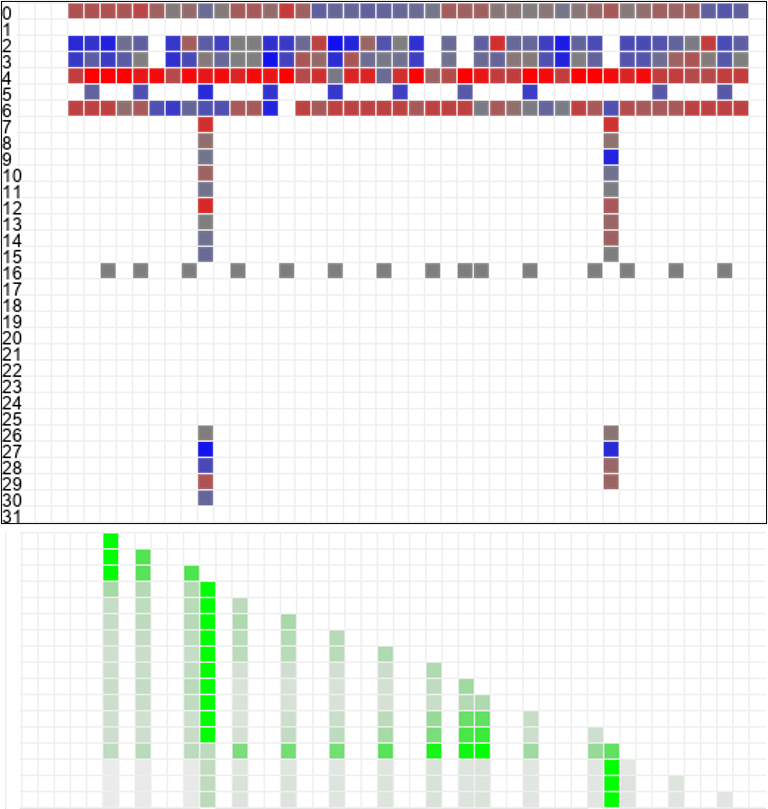
\includegraphics{images/example.png}}
    \caption{Magnetization as a function of applied field.
    It is good practice to explain the significance of the figure in the caption.}
    \label{fig2}
\end{figure}



\subsection{Learned representions}  

% \begin{figure*}[!t]
%     \centerline{\includesvg[inkscapelatex=false,width=2\columnwidth]{images/tsne.svg}}    
%     \caption{Magnetization as a function of applied field.
%     It is good practice to explain the significance of the figure in the caption.}
%     \label{fig1}
%     \end{figure*}


% \begin{figure*}[!h]

%     \centerline{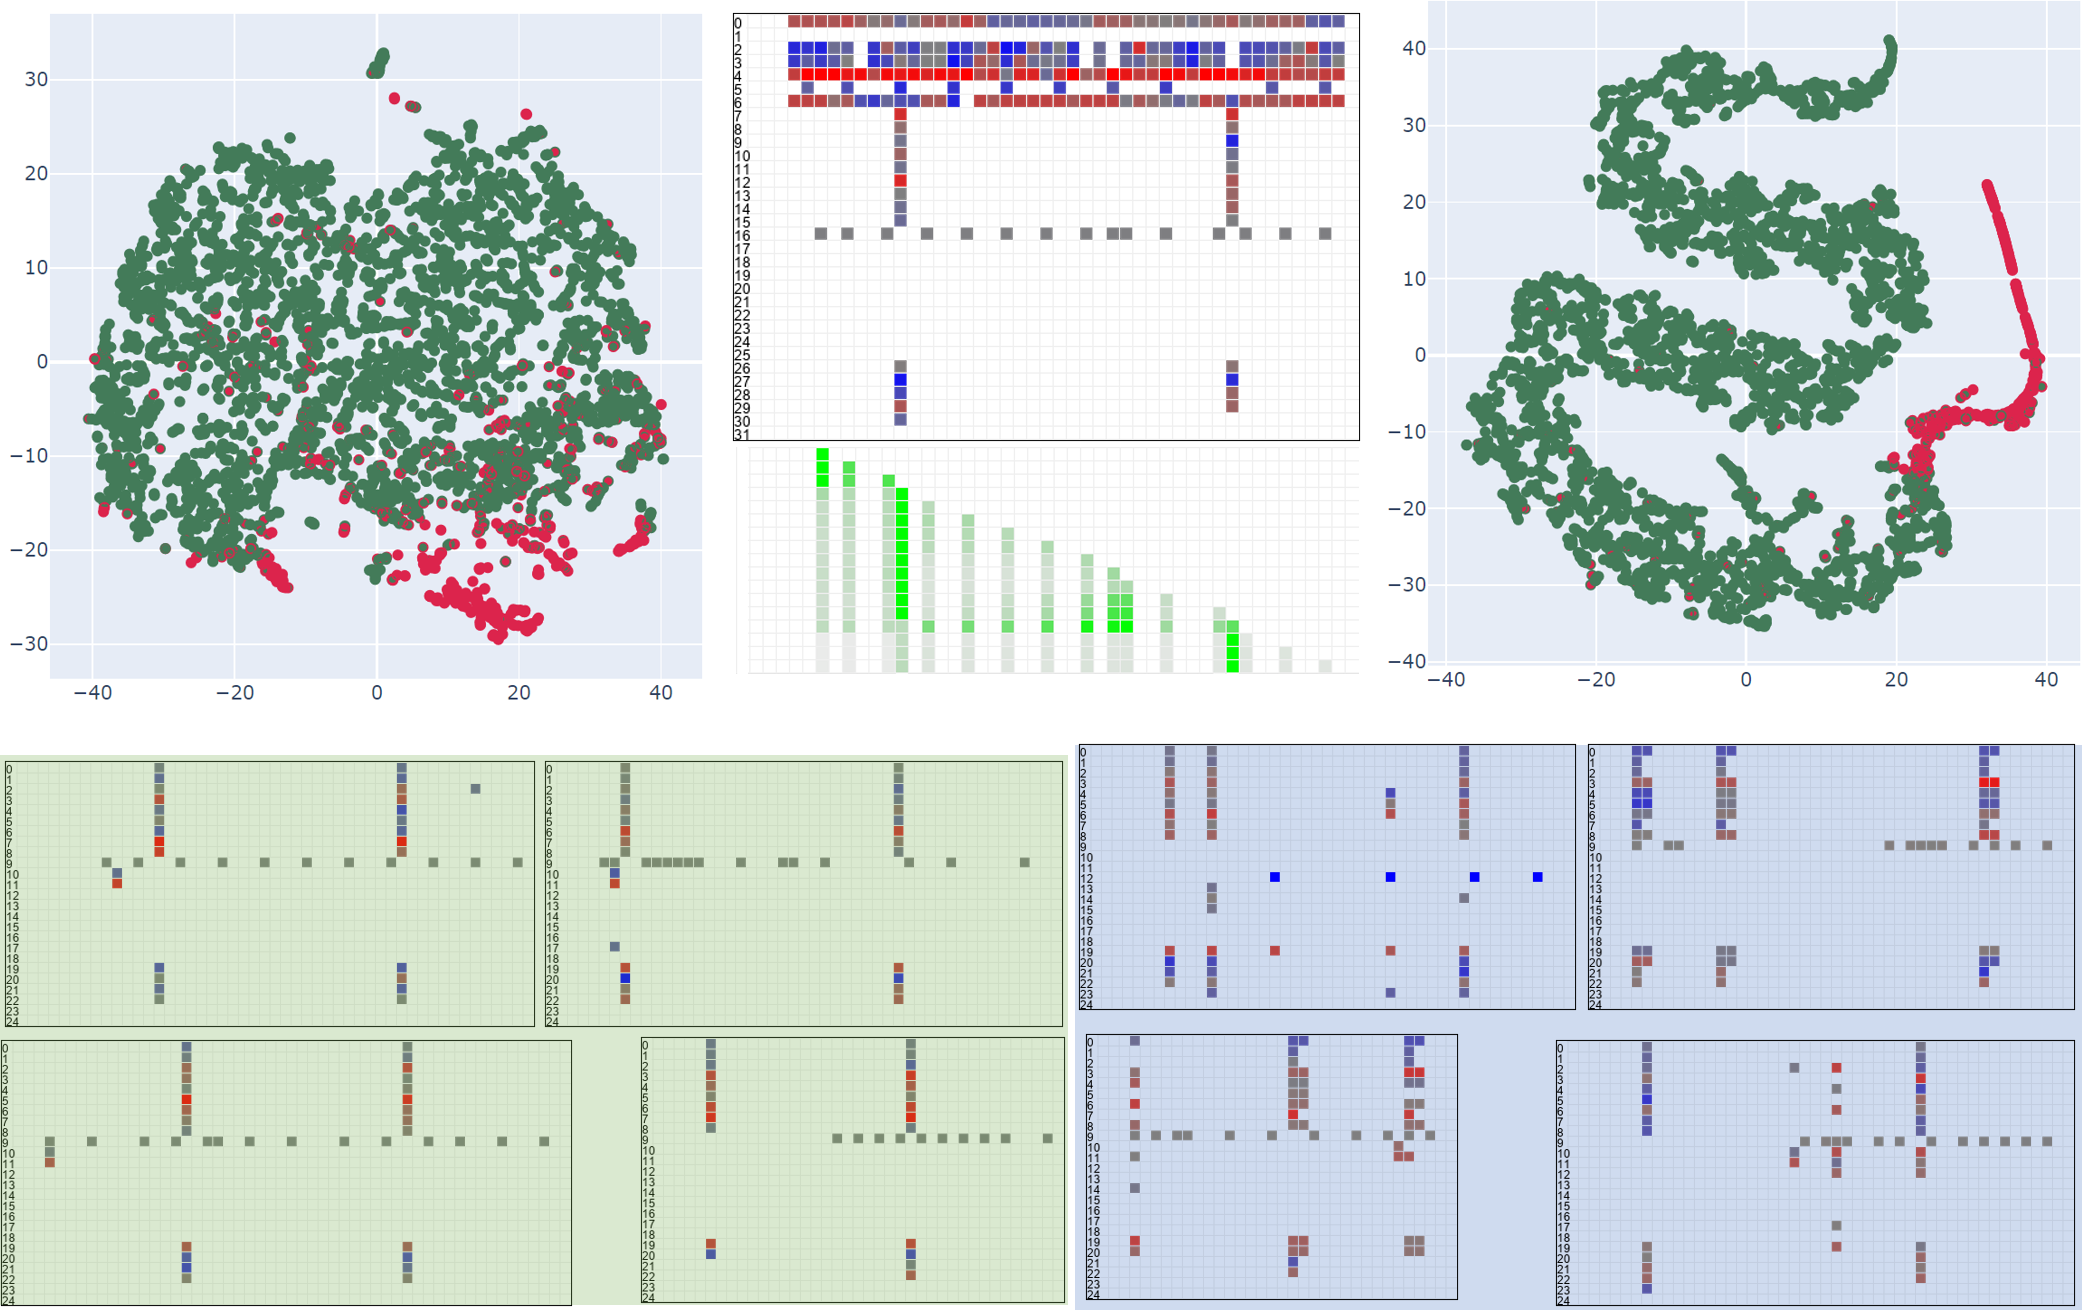
\includegraphics{images/tsne.png}}
%     \caption{Magnetization as a function of applied field.
%     It is good practice to explain the significance of the figure in the caption.}
%     \label{fig2}
%     \end{figure*}






We have visualized the learned patients' embeddings for an example dataset and setting (P12-seft). Fig. 1-a and b visualize the t-SNE plot for the learned representations of TEE+DAM and TEE, respectively.     


\begin{figure}[!h]

    \centerline{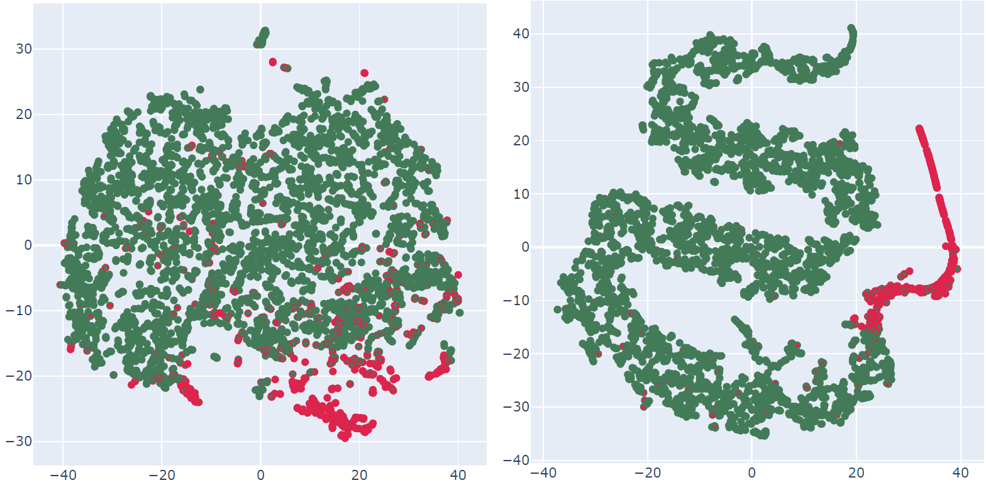
\includegraphics{images/small_tsne.png}}
    \caption{Magnetization as a function of applied field.
    It is good practice to explain the significance of the figure in the caption.}
    \label{fig2}
\end{figure}

The 10 nearest neighbor pattern similarity (10-nnps) of positive labels for TEE+DAM ($0.903 \pm 0.058 $) is significantly higher than (DAM) ($0.832 \pm 0.095$)($pvalue \leq 0.001$). The sampling pattern of an example patient and its 4 nearest neighbors (in the embedding space) is visualized in Fig. \ref*{fig2}-c and d for TEE+DAM and TEE, respectively. As can be seen, in TEE+DAM, the 4 neighbors have a more similar pattern compared to the example patient. 


\begin{figure}[!h]

    \centerline{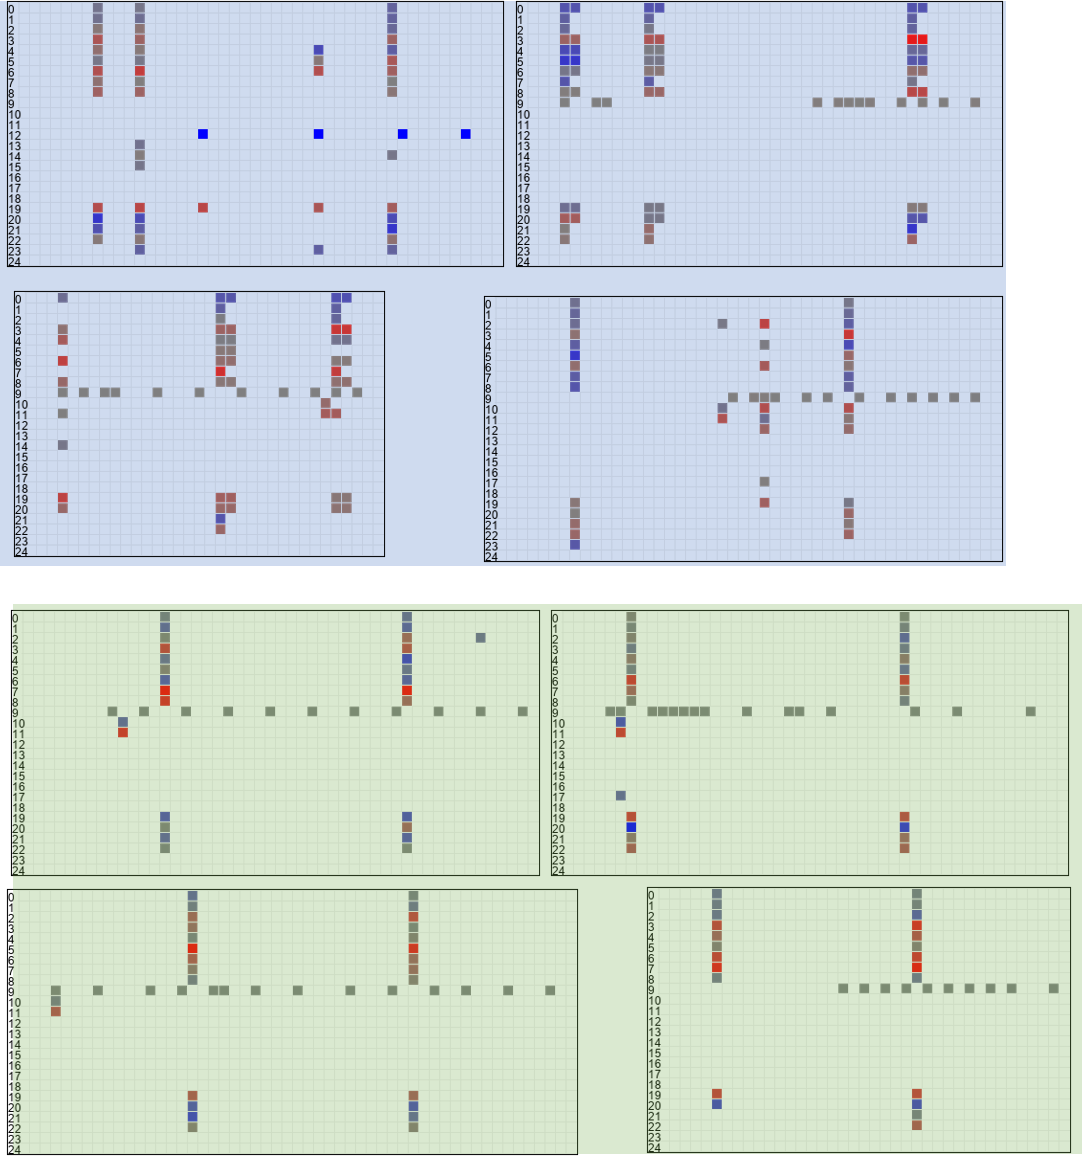
\includegraphics{images/knn_patterns.png}}
    
    \caption{Magnetization as a function of applied field.
    It is good practice to explain the significance of the figure in the caption.}
    \label{fig2}
\end{figure}

We argue that event encoding could lead to better representation learning in EHRs although it does not necessarily leads to better performance. Patient representation that can respect the irregular sampling pattern in EHRs could have various applications in synthetic data generation..





\section{Conclusion}
\label{sec:Conclusion}

data generation with similar patterns

pattern similarity index






% \begin{thebibliography}{00}

% \bibitem{b1} G. O. Young, ``Synthetic structure of industrial plastics,'' in \emph{Plastics,} 2\textsuperscript{nd} ed., vol. 3, J. Peters, Ed. New York, NY, USA: McGraw-Hill, 1964, pp. 15--64.

% \bibitem{b2} W.-K. Chen, \emph{Linear Networks and Systems.} Belmont, CA, USA: Wadsworth, 1993, pp. 123--135.

% \bibitem{b3} J. U. Duncombe, ``Infrared navigation---Part I: An assessment of feasibility,'' \emph{IEEE Trans. Electron Devices}, vol. ED-11, no. 1, pp. 34--39, Jan. 1959, 10.1109/TED.2016.2628402.

% \bibitem{b4} E. P. Wigner, ``Theory of traveling-wave optical laser,'' \emph{Phys. Rev}., vol. 134, pp. A635--A646, Dec. 1965.

% \bibitem{b5} E. H. Miller, ``A note on reflector arrays,'' \emph{IEEE Trans. Antennas Propagat}., to be published.

% \bibitem{b6} E. E. Reber, R. L. Michell, and C. J. Carter, ``Oxygen absorption in the earth's atmosphere,'' Aerospace Corp., Los Angeles, CA, USA, Tech. Rep. TR-0200 (4230-46)-3, Nov. 1988.

% \bibitem{b7} J. H. Davis and J. R. Cogdell, ``Calibration program for the 16-foot antenna,'' Elect. Eng. Res. Lab., Univ. Texas, Austin, TX, USA, Tech. Memo. NGL-006-69-3, Nov. 15, 1987.

% \bibitem{b8} \emph{Transmission Systems for Communications}, 3\textsuperscript{rd} ed., Western Electric Co., Winston-Salem, NC, USA, 1985, pp. 44--60.

% \bibitem{b9} \emph{Motorola Semiconductor Data Manual}, Motorola Semiconductor Products Inc., Phoenix, AZ, USA, 1989.

% \bibitem{b10} G. O. Young, ``Synthetic structure of industrial
% plastics,'' in Plastics, vol. 3, Polymers of Hexadromicon, J. Peters,
% Ed., 2\textsuperscript{nd} ed. New York, NY, USA: McGraw-Hill, 1964, pp. 15-64.
% [Online]. Available:
% \underline{http://www.bookref.com}.

% \bibitem{b11} \emph{The Founders' Constitution}, Philip B. Kurland
% and Ralph Lerner, eds., Chicago, IL, USA: Univ. Chicago Press, 1987.
% [Online]. Available: \underline{http://press-pubs.uchicago.edu/founders/}

% \bibitem{b12} The Terahertz Wave eBook. ZOmega Terahertz Corp., 2014.
% [Online]. Available:
% \underline{http://dl.z-thz.com/eBook/zomega\_ebook\_pdf\_1206\_sr.pdf}. Accessed on: May 19, 2014.

% \bibitem{b13} Philip B. Kurland and Ralph Lerner, eds., \emph{The
% Founders' Constitution.} Chicago, IL, USA: Univ. of Chicago Press,
% 1987, Accessed on: Feb. 28, 2010, [Online] Available:
% \underline{http://press-pubs.uchicago.edu/founders/}

% \bibitem{b14} J. S. Turner, ``New directions in communications,'' \emph{IEEE J. Sel. Areas Commun}., vol. 13, no. 1, pp. 11-23, Jan. 1995.

% \bibitem{b15} W. P. Risk, G. S. Kino, and H. J. Shaw, ``Fiber-optic frequency shifter using a surface acoustic wave incident at an oblique angle,'' \emph{Opt. Lett.}, vol. 11, no. 2, pp. 115--117, Feb. 1986.

% \bibitem{b16} P. Kopyt \emph{et al., ``}Electric properties of graphene-based conductive layers from DC up to terahertz range,'' \emph{IEEE THz Sci. Technol.,} to be published. DOI: 10.1109/TTHZ.2016.2544142.

% \bibitem{b17} PROCESS Corporation, Boston, MA, USA. Intranets:
% Internet technologies deployed behind the firewall for corporate
% productivity. Presented at INET96 Annual Meeting. [Online].
% Available: \underline{http://home.process.com/Intranets/wp2.htp}

% \bibitem{b18} R. J. Hijmans and J. van Etten, ``Raster: Geographic analysis and modeling with raster data,'' R Package Version 2.0-12, Jan. 12, 2012. [Online]. Available: \underline {http://CRAN.R-project.org/package=raster} 

% \bibitem{b19} Teralyzer. Lytera UG, Kirchhain, Germany [Online].
% Available:
% \underline{http://www.lytera.de/Terahertz\_THz\_Spectroscopy.php?id=home}, Accessed on: Jun. 5, 2014

% \bibitem{b20} U.S. House. 102\textsuperscript{nd} Congress, 1\textsuperscript{st} Session. (1991, Jan. 11). \emph{H. Con. Res. 1, Sense of the Congress on Approval of}  \emph{Military Action}. [Online]. Available: LEXIS Library: GENFED File: BILLS

% \bibitem{b21} Musical toothbrush with mirror, by L.M.R. Brooks. (1992, May 19). Patent D 326 189 [Online]. Available: NEXIS Library: LEXPAT File: DES

% \bibitem{b22} D. B. Payne and J. R. Stern, ``Wavelength-switched pas- sively coupled single-mode optical network,'' in \emph{Proc. IOOC-ECOC,} Boston, MA, USA, 1985, pp. 585--590.

% \bibitem{b23} D. Ebehard and E. Voges, ``Digital single sideband detection for interferometric sensors,'' presented at the \emph{2\textsuperscript{nd} Int. Conf. Optical Fiber Sensors,} Stuttgart, Germany, Jan. 2-5, 1984.

% \bibitem{b24} G. Brandli and M. Dick, ``Alternating current fed power supply,'' U.S. Patent 4 084 217, Nov. 4, 1978.

% \bibitem{b25} J. O. Williams, ``Narrow-band analyzer,'' Ph.D. dissertation, Dept. Elect. Eng., Harvard Univ., Cambridge, MA, USA, 1993.

% \bibitem{b26} N. Kawasaki, ``Parametric study of thermal and chemical nonequilibrium nozzle flow,'' M.S. thesis, Dept. Electron. Eng., Osaka Univ., Osaka, Japan, 1993.

% \bibitem{b27} A. Harrison, private communication, May 1995.

% \bibitem{b28} B. Smith, ``An approach to graphs of linear forms,'' unpublished.

% \bibitem{b29} A. Brahms, ``Representation error for real numbers in binary computer arithmetic,'' IEEE Computer Group Repository, Paper R-67-85.

% \bibitem{b30} IEEE Criteria for Class IE Electric Systems, IEEE Standard 308, 1969.

% \bibitem{b31} Letter Symbols for Quantities, ANSI Standard Y10.5-1968.

% \bibitem{b32} R. Fardel, M. Nagel, F. Nuesch, T. Lippert, and A. Wokaun, ``Fabrication of organic light emitting diode pixels by laser-assisted forward transfer,'' \emph{Appl. Phys. Lett.}, vol. 91, no. 6, Aug. 2007, Art. no. 061103.~

% \bibitem{b33} J. Zhang and N. Tansu, ``Optical gain and laser characteristics of InGaN quantum wells on ternary InGaN substrates,'' \emph{IEEE Photon. J.}, vol. 5, no. 2, Apr. 2013, Art. no. 2600111

% \bibitem{b34} S. Azodolmolky~\emph{et al.}, Experimental demonstration of an impairment aware network planning and operation tool for transparent/translucent optical networks,''~\emph{J. Lightw. Technol.}, vol. 29, no. 4, pp. 439--448, Sep. 2011.

% \end{thebibliography}

\printbibliography




% \begin{IEEEbiography}[{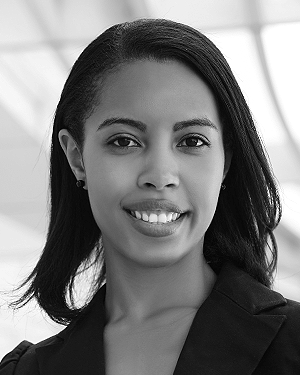
\includegraphics[width=1in,height=1.25in,clip,keepaspectratio]{a1.png}}]{First A. Author} (M'76--SM'81--F'87) and all authors may include 
% biographies. Biographies are often not included in conference-related
% papers. This author became a Member (M) of IEEE in 1976, a Senior
% Member (SM) in 1981, and a Fellow (F) in 1987. The first paragraph may
% contain a place and/or date of birth (list place, then date). Next,
% the author's educational background is listed. The degrees should be
% listed with type of degree in what field, which institution, city,
% state, and country, and year the degree was earned. The author's major
% field of study should be lower-cased. 

% The second paragraph uses the pronoun of the person (he or she) and not the 
% author's last name. It lists military and work experience, including summer 
% and fellowship jobs. Job titles are capitalized. The current job must have a 
% location; previous positions may be listed 
% without one. Information concerning previous publications may be included. 
% Try not to list more than three books or published articles. The format for 
% listing publishers of a book within the biography is: title of book 
% (publisher name, year) similar to a reference. Current and previous research 
% interests end the paragraph. The third paragraph begins with the author's 
% title and last name (e.g., Dr.\ Smith, Prof.\ Jones, Mr.\ Kajor, Ms.\ Hunter). 
% List any memberships in professional societies other than the IEEE. Finally, 
% list any awards and work for IEEE committees and publications. If a 
% photograph is provided, it should be of good quality, and 
% professional-looking. Following are two examples of an author's biography.
% \end{IEEEbiography}

% \begin{IEEEbiography}[{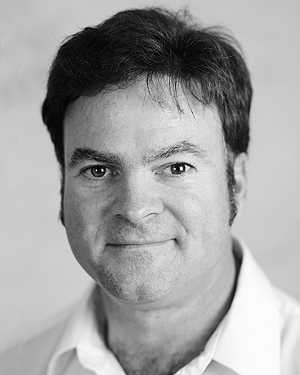
\includegraphics[width=1in,height=1.25in,clip,keepaspectratio]{a2.png}}]{Second B. Author} was born in Greenwich Village, New York, NY, USA in 
% 1977. He received the B.S. and M.S. degrees in aerospace engineering from 
% the University of Virginia, Charlottesville, in 2001 and the Ph.D. degree in 
% mechanical engineering from Drexel University, Philadelphia, PA, in 2008.

% From 2001 to 2004, he was a Research Assistant with the Princeton Plasma 
% Physics Laboratory. Since 2009, he has been an Assistant Professor with the 
% Mechanical Engineering Department, Texas A{\&}M University, College Station. 
% He is the author of three books, more than 150 articles, and more than 70 
% inventions. His research interests include high-pressure and high-density 
% nonthermal plasma discharge processes and applications, microscale plasma 
% discharges, discharges in liquids, spectroscopic diagnostics, plasma 
% propulsion, and innovation plasma applications. He is an Associate Editor of 
% the journal \emph{Earth, Moon, Planets}, and holds two patents. 

% Dr. Author was a recipient of the International Association of Geomagnetism 
% and Aeronomy Young Scientist Award for Excellence in 2008, and the IEEE 
% Electromagnetic Compatibility Society Best Symposium Paper Award in 2011. 
% \end{IEEEbiography}

% \begin{IEEEbiography}[{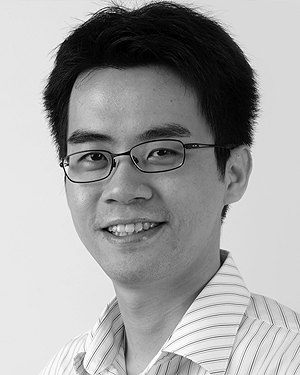
\includegraphics[width=1in,height=1.25in,clip,keepaspectratio]{a3.png}}]{Third C. Author, Jr.} (M'87) received the B.S. degree in mechanical 
% engineering from National Chung Cheng University, Chiayi, Taiwan, in 2004 
% and the M.S. degree in mechanical engineering from National Tsing Hua 
% University, Hsinchu, Taiwan, in 2006. He is currently pursuing the Ph.D. 
% degree in mechanical engineering at Texas A{\&}M University, College 
% Station, TX, USA.

% From 2008 to 2009, he was a Research Assistant with the Institute of 
% Physics, Academia Sinica, Tapei, Taiwan. His research interest includes the 
% development of surface processing and biological/medical treatment 
% techniques using nonthermal atmospheric pressure plasmas, fundamental study 
% of plasma sources, and fabrication of micro- or nanostructured surfaces. 

% Mr. Author's awards and honors include the Frew Fellowship (Australian 
% Academy of Science), the I. I. Rabi Prize (APS), the European Frequency and 
% Time Forum Award, the Carl Zeiss Research Award, the William F. Meggers 
% Award and the Adolph Lomb Medal (OSA).
% \end{IEEEbiography}

\end{document}
